% !TeX spellcheck = it_IT
%Insomma: 
%4 lezioni sugli attacchi low level
%4 lezioni sulle difese low level
%5 lezioni su fuzzing, side channel, symbolic execution, analisi di programmi
%TL;DR: attacco, difesa, analisi
\section{Spatial Memory Errors}
%Slide 0 Buffer Overflow - Intro

Ci concentriamo su linguaggi low level (e.g., C), i quali tendono a crashare in caso di errori (come buffer overflow), ma un attaccante può \textbf{sfruttare le vulnerabilità} per ottenere informazioni (e.g., Heartbleed, bug SSL che permetteva di leggere tutta la memoria del programma, che su SSL insomma, peso), corrompere memoria, fino ad arbitrary code execution (la macchina comincia ad eseguire altro, diventa una "weird machine"), ecc.\\
Il crash (ovvero \texttt{segfault}), se analizzato può portare ad un attacco, anche se non tutti i casi sono exploitabili (molti sì).\\

Questo tipo di bug hanno una lunga storia e sono tuttora presenti, e lo saranno finché C e C++ saranno usati. Inoltre è utile studiare l'evoluzione del bug stesso, assieme alle difese create per contrastarlo. Alcune caratteristiche di un attacco/difesa possono risultare presenti anche in altri attacchi.\\

Inoltre, solitamente, l'attacco è molto più semplice della difesa. Per l'attacco mi basta un punto, per la difesa devo essere sicuro di aver coperto tutti i possibili punti di attacco, senza degradare troppo le performance.\\

I sistemi C e C++ sono ancora molto presenti e spesso sono parte di sistemi critici come: 
\begin{itemize}
	\item OS, Kernel e relative utilities
	\item Server che richiedono alte prestazioni (Apache httpd, nginx, MySQL, redis)
	\item Sistemi embedded (risorse limitate, le performance sono importanti)
\end{itemize}

La prima versione di buffer overflow funzionante è del 1988: Morris Worm, per poi dare inizio ad una catena di exploit che permettono la compromissione della macchina stessa (a diversi livelli), in qualsiasi caso con un impatto significativo.\\

\newpage

%Slide 1 Buffer Overflow - Memory Layout
\subsection{Memory Layout}
Dobbiamo sapere come un programma viene caricato in memoria, in quali zone e di conseguenza cos'è lo stack e quali sono gli effetti delle chiamate a funzione. Parleremo del modello Linux \texttt{x64}, anche se il concetto dell'attacco è universale l'implementazione può cambiare in base a dettagli tecnici (architectural dependent).\\

\textbf{Ogni processo} ha un proprio \textbf{layout di memoria}, con indirizzi che vanno da \texttt{0x00000000} a \texttt{0xffffffff} (per 32 bit, con 64 sarebbero troppo lunghi da scrivere), quindi 4GB di indirizzamento totali.\\

Linux divide:
\begin{itemize}
	\item 1GB per il sistema operativo, dall'alto
	\item 3GB per le applicazioni
\end{itemize}
Di conseguenza il primo indirizzo valido per il programma è \texttt{0xbfffffff}, sopra c'è il kernel.\\

Il \textbf{loader carica in memoria} un \textbf{processo} quando questo viene chiamato, occupando la page table ed allestendo la memoria per l'uso del programma. \\

\newpage

Il loader divide la memoria (tra quella adibita al programma, i 3GB di prima) in sezioni:
\begin{itemize}
	\item \textbf{Text} per memorizzare il codice del programma
	\item Zone per dati inizializzati (\textbf{Data}) e non (Block Started by Symbol \textbf{BSS})
\end{itemize}
Queste sono \textbf{conosciute a compile time}, mentre
\begin{itemize}
	\item \textbf{Stack}
	\item \textbf{Heap}
\end{itemize}
Sono \textbf{dinamiche} e permettono la gestione del programma.
\begin{center}
	\includegraphics[width=0.85\linewidth]{img/sme/memory_all1}
\end{center}

Stack e Heap quindi sono zone dinamiche che \textbf{crescono in direzioni opposte} (stack verso il basso).\\
Nell'heap ci sono le allocazioni dinamiche effettuate dal programmatore stesso (\texttt{malloc} e simili), mentre lo \textbf{stack} viene \textbf{gestito dal compilatore} per memorizzare cose come le chiamate a funzione. \\

\newpage

\subsubsection{Stack}
All'interno dello stack viene gestita l'esecuzione del programma. Gli \textbf{indirizzi dello stack crescono verso il basso}, partendo da \texttt{0xbfffffff} e scendono. Questo rende possibile l'attacco di buffer overflow stack based, nel modo attualmente esistente.\\

Man mano che viene allocata memoria, lo stack alloca spazio dall'alto verso il basso. \texttt{Push} decrementa il valore dell'indirizzo, \texttt{Pop} lo aumenta.\\

\paragraph{Stack Pointer:} Su architetture Intel, si tratta del \textbf{registro} che tiene conto dell'\textbf{indirizzo a cui è arrivato lo stack}, il valore dello spazio allocato più in basso (ultimo valore allocato, da dove posso ricominciare ad allocare).\\

Il compilatore utilizza lo stack quando vengono chiamate le funzioni, \textbf{nel momento in cui avviene una chiamata a funzione}:
\begin{itemize}
	\item viene effettuata la \texttt{push} (istruzione macchina) dei parametri della funzione sullo stack
	\item l'istruzione macchina \texttt{call} viene chiamata, portando l'esecuzione all'indirizzo di memoria del codice della funzione
	\item la \texttt{call} effettua anche la \texttt{push} sullo stack dell'indirizzo di ritorno di una funzione, ovvero da dove proseguire l'esecuzione al termine della funzione 
\end{itemize} 
%Viene effettuata la push e poi la call? Check

Dopo queste istruzioni comincia l'esecuzione della funzione. All'\textbf{interno dello stack} vengono \textbf{memorizzate le variabili locali}, quindi viene effettuata una \texttt{push} di queste variabili all'interno dello stack.\\

\newpage

Al termine dell'esecuzione ci sarà un'istruzione \texttt{ret} che fa tornare l'\textbf{esecuzione all'indirizzo puntato dal return address} memorizzato in precedenza sullo stack (anche senza \texttt{return} esplicito, serve a continuare l'esecuzione del programma dopo la funzione).\\

La funzione di \texttt{ret}: 
\begin{itemize}
	\item libera la zona dedicata alle variabili locali, \texttt{pop} di tutte le variabili memorizzate sullo stack
	\item carica nell'instruction pointer (o program counter, registro che tiene traccia dell'istruzione da eseguire) il valore del return address (indirizzo della prossima istruzione che deve eseguire il processore)
\end{itemize}
Bisogna deallocare anche i parametri allocati sullo stack ma chi lo effettua dipende dalla calling convention del compilatore, quindi può farlo il chiamato o il chiamante (i.e., il pop di quei valori verrà effettuato prima o dopo il \texttt{ret}).\\

In ordine, dall'alto verso il basso, all'interno dello stack saranno presenti: 
\begin{itemize}
	\item Parametri 
	\item Return address
	\item Variabili locali
\end{itemize}

\newpage

\subsection{Stack-based Overflow}

Esempio di bug: 
\begin{minted}{c}
void f (par){
	char buf[10];
	strcpy(buf, par);
}
\end{minted}

La funzione \textbf{non controlla dimensioni di sorgente e destinazione}, quindi cosa succede se l'\textbf{elemento da copiare è più grande} della \textbf{memoria} che gli è stata \textbf{allocata} (ovvero la dimensione del buffer destinazione)?\\

Lo \textbf{stack} sarà \textbf{composto da}:
\begin{itemize}
	\item parametri della funzione, \texttt{par} in questo caso
	\item return address
	\item variabili locali, qui solo il buffer destinazione
\end{itemize} 

Se la dimensione del buffer da copiare è maggiore del buffer allocato il programma \textbf{andrà a sovrascrivere i valori precedenti nello stack} (lo stack alloca dall'alto verso il basso, ma gli indirizzi del buffer vanno dal basso verso l'alto, l'indice 1 è più in basso dell'indice 8, per mantenere coerente l'aritmetica con i puntori, I guess). \\

Il valore sopra il buffer nello stack è il return address, che porterà a tornare ad un indirizzo casuale se sovrascritto, portando ad un \texttt{segfault}.\\

Non c'è un controllo che limiti la scrittura alla dimensione del buffer, portando a sovrascrivere altre parti dello stack.\\

\newpage

\subsubsection{Code Injection}
Come possiamo sfruttare questa situazione? Tramite buffer overflow posso avere il controllo sul return address; control flow hijacking.\\

Per arrivare ad \textbf{eseguire codice arbitrario} devo
\begin{itemize}
	\item definire il codice
	\item iniettarlo in memoria
	\item cambiare il valore del return address in modo che punti a quella zona di memoria
\end{itemize}

\paragraph{Definire il codice:} Il processore legge solamente stringhe di byte che corrispondono alle istruzioni da eseguire. Noi dobbiamo costruire un bytestream a partire da del codice sorgente che vogliamo eseguire. Un bytestream che chiama \texttt{/bin/bash} diventa uno shellcode.\\
Dobbiamo forgiare un bytestream adatto alle nostre esigenze, manualmente prendendolo da del codice eseguito o tramite tool appositi (più facile solitamente).

\paragraph{Injection Vector:} Per metterlo in memoria, il posto ideale sarebbe il \textbf{buffer} che abbiamo \textbf{già a disposizione}. L'\textbf{input} viene \textbf{copiato nel buffer}, il quale è sullo stack. Quindi inserendo il bytestream all'interno dell'input posso inserirlo in memoria all'interno del buffer.\\

Dobbiamo \textbf{costruire un input} che fa partire l'esecuzione del codice voluto (chiamato injection vector). Sarà quindi composto dal \textbf{bytestream del codice} (e.g., shellcode) e dal \textbf{valore che sovrascriverà il return address}, ovvero l'indirizzo del buffer (come trovarlo?). \\
Nell'esempio sopra ci saranno 10 byte per lo shellcode (dimensione allocata per il buffer) e 4 byte per il return address (considerando architetture a 32 bit).\\
In questo modo, quando il programma torna dalla funzione, porrà nel program counter l'indirizzo del buffer, contenente il bytestream forgiato da noi. La sequenza di istruzioni posta nel buffer sarà quindi interpretata come codice. Abbiamo dirottato il control flow, portando all'esecuzione di codice arbitrario.\\

\paragraph{Spatial memory error:} Stiamo "mischiando" dati dell'utente e control channel (comandi di controllo), problematica comune a più vulnerabilità e possibili ambiti. Sovrascriviamo nello spazio dei caratteri di controllo. L'esecuzione di codice arbitrario avviene al ritorno della funzione vulnerabile.\\

Adesso ci sono protezioni che bloccano esecuzione di codice all'interno dello stack, non è una zona di memoria che dovrebbe contenere codice (anche se ci sono anche casi particolari) e l'esecuzione di codice presente in zone di memoria simili è bloccata.\\

%End L1

\newpage

\subsection{Heap}

\subsubsection{Heap vs Stack}
Lo \textbf{stack} è principalmente gestito dal compilatore per allocazioni \textbf{statiche} della memoria, conosciute a compile time. Inoltre tutti i metadati utili al programma sono memorizzati sullo stack. Un esempio di metadato è il return address per il ritorno di una funzione. \\

Questo è solitamente nascosto al programmatore, se la dimensione dei dati non è nota a priori viene usato l'\textbf{heap}, una memoria comandata (allocazione e liberazione) dal programmatore tramite funzioni di libreria. Generalmente più lenta ed a \textbf{gestione manuale}.  Solitamente usato per oggetti, structs ed in generale elementi più grandi.\\

Lo stack cresce dell'alto verso il basso (indirizzi), mentre l'heap cresce dal basso verso l'alto. Una \texttt{push} sullo stack sposta il \texttt{rsp} verso il basso (e, di conseguenza, la \texttt{pop} verso l'alto). In caso di un utilizzo troppo elevato di memoria si possono "incontrare" le due zone (hai finito la memoria).\\

La vulnerabilità già vista sullo stack nasce dal "mischiare" dati inseriti dall'utente con metadati che permettono di alterare il flusso di controllo del programma.\\

le due funzioni principali per gestire la memoria nell'heap sono: 
\begin{itemize}
	\item \texttt{malloc(size)}: restituisce un puntatore ad una zona di memoria con dimensione \texttt{size}
	\item \texttt{free(ptr)}: dato un puntatore, libera la zona di memoria associata
\end{itemize}

%\subsubsection{Heap overflow}
Anche nell'heap sono presenti metadati, e di conseguenza la possibilità di sovrascriverli, portando a possibili vulnerabilità.\\

\paragraph{Allocatori:} Definiti nelle librerie di sistema, per gestire le zone di memoria allocate servono comunque dei metadati. L'allocatore gestisce i propri dati all'interno dell'heap stesso (problema di canale).

\newpage

\subsubsection{Heap Chunk} 

\paragraph{Heap Chunk:} Struttura dati per la memoria nell'heap. Struttura:
\begin{minted}{c}
struct malloc_chunk {
	INTERNAL_SIZE_T 	prev_size; 
	INTERNAL_SIZE_T 	size; 
	
	struct malloc_chunk* 	fd;
	struct malloc_chunk* 	bk;
	
	struct malloc_chunk* 	fd_nextsize;
	struct malloc_chunk* 	bk_nextsize;
	};
\end{minted}
I ordine, i parametri sono:
\begin{itemize}
	\item \texttt{prev\_size}: dimensione della zona di memoria precedente, usato solo se il chunk è libero
	\item \texttt{size}: dimensione della zona di memoria occupata da questo chunk, overhead compreso
	\item \texttt{fd}, \texttt{bk}: puntatori alle zone di memoria precedenti e successive nella lista di chunk liberi (e di conseguenza presenti solo se il blocco è libero)
	\item \texttt{fd\_nextsize}, \texttt{bk\_nextsize}: puntatori alle dimensioni degli elementi adiacenti nella lista di chunk liberi (usati solo se il chunk è libero)
\end{itemize}
\begin{center}
	\includegraphics[width=\linewidth]{img/sme/heapchunk}
\end{center}
I chunk occupati contengono solo \texttt{size} e i dati. Il puntatore di ritorno ottenuto tramite \texttt{malloc} punta all'inizio della zona contenente i dati. \\

\newpage

\subsubsection{Allocare e deallocare memoria}

\paragraph{Allocazione:} All'inizio dell'esecuzione si ha un top chunk, che rappresenta tutta la grandezza dell'heap. Si ha un puntatore al top chunk chiamato \texttt{av\_top}; inizialmente questo puntatore coincide con la base della memoria. In seguito ad una \texttt{malloc}, viene allocata la zona di memoria richiesta, restituendo i relativi puntatori, e di conseguenza  \texttt{av\_top} viene spostato "sopra" al blocco allocato, deve puntare sempre alla zona di memoria "rimanente"; il top chunk decresce in seguito all'allocazione.\\

\paragraph{Deallocazione:} Oltre allo spazio libero del top chunk sono presenti delle liste di free chunk, una per ogni dimensione di chunk liberi (se posso occupare la memoria esatta lo faccio, serve a ridurre la frammentazione). Quando viene richiesta un'allocazione, prima cerca se c'è una zona di memoria "grande giusta" (o poco più, se mi servono 256 byte cerco nella lista di blocchi liberi da 256 byte), se non c'è una zona adatta nelle liste di chunk liberi allora prende la memoria dal top chunk.\\

Nel caso in cui due chunk adiacenti diventino liberi, vengono collassati in uno solo e lo inserisce nella lista rilevante.\\

\vfill

\begin{minipage}{0.43\textwidth}
	\textbf{Allocazione:}
	\begin{itemize}
		\item Richiesta di memoria (\texttt{malloc})
		\item Ricerca di un blocco libero (prima dalle liste, eventualmente si usa il top chunk)
		\item Aggiornamento della struttura di gestione (metadati)
		\item Restituzione del puntatore
	\end{itemize}
\end{minipage}
\hfill
\begin{minipage}{0.43\textwidth}
	\textbf{Deallocazione:}
	\begin{itemize}
		\item Richiesta di rilascio (\texttt{free})
		\item Il blocco viene marcato come libero 
		\item Coalescenza di blocchi adiacenti (se presenti, si fondono blocchi liberi adiacenti in uno solo)
		\item Aggiornamento della struttura di gestione
	\end{itemize}
\end{minipage}

\newpage

\subsection{Heap Overflow}

\subsubsection{Unlink}
Quando viene effettuata una allocazione bisogna aggiornare i puntatori, il nodo occupato va "sganciato" dalla lista (doppiamente concatenata) di blocchi liberi, e di conseguenza i puntatori del blocco successivo e precedente vanno aggiornati (sai come si rimuove un elemento da una lista dai). La procedura è
\begin{minted}{c}
void unlink(malloc_chunk *P, malloc_chunk *BK, 
	malloc_chunk *FD) {
		FD = P->fd;
		BK = P->bk;
		FD->bk = BK;
		BK->fd = FD;
}
\end{minted}
Dove: 
\begin{itemize}
	\item \texttt{P} nodo da eliminare
	\item \texttt{BK} nodo precedente
	\item \texttt{FD} nodo successivo 
\end{itemize}
"Stacco" il nodo da eliminare facendo puntare il puntatore \texttt{bk} del nodo successivo al nodo precedente e viceversa.\\

\newpage

\subsubsection{Exploit "Naive"}
Se non è presente nessun controllo durante le scritture, una write troppo grande può andare a sovrascrivere i chunk (liberi o occupati) superiori, metadati compresi.\\

Nello specifico, posso sovrascrivere il \texttt{FD->bk} e \texttt{P->bk}, rispettivamente con l'indirizzo di un return address e un indirizzo di un buffer (injection vector).\\
\begin{minted}{c}
	FD->bk = return address address;
	FD = P->fd;
	BK = P->bk = address of the buffer;
	FD->bk = BK;
\end{minted}

Partendo da un heap con dei chunk liberi e la relativa lista, facendo overflow in un chunk occupato sottostante si può sovrascrivere il puntatore \texttt{bk} di due chunk vuoti con indirizzi determinati dall'attaccante (rispettivamente, un blocco con inizio di un buffer con codice malevolo, il blocco dopo con l'indirizzo del return address di una funzione).\\

Quando il programma andrà ad allocare il primo dei blocchi con i valori sovrascritti dovrà rimuoverlo dalla lista di blocchi liberi, quindi eseguire la procedura di unlink: il \texttt{bk} del blocco "sganciato" punta al buffer contenente qualcosa (e.g., shellcode, inizio di un buffer controllato dall'attaccante, in qualsiasi modo), mentre il \texttt{bk} blocco successivo punta al return address di una funzione, il quale verrà sovrascritto con l'indirizzo del buffer (procedura di unlink), portando il programma ad eseguire il codice all'interno del buffer una volta che il programma dovrà seguire il return address sovrascritto.\\

Questo exploit è stato patchato controllando che \texttt{FD} e \texttt{BK} puntino effettivamente l'uno all'altro, non si può più sparare allo stack.\\

%up to s11
% Missing House of Force attack

\newpage

\subsubsection{House of Force}

Dopo la patch per la correzione dell'unlink sono nate nuove tecniche per sfruttare l'heap overflow, le principali si chiamano:
\begin{itemize}
	\item The House of Prime
	\item The House of Mind
	\item \textbf{The House of Force}
	\item The House of Lore
	\item The House of Spirit
	\item The House of Chaos
\end{itemize}

Verrà mostrata solo la House of Force, spiegazioni ed esempi per le altre possono essere trovate \href{https://github.com/shellphish/how2heap}{\texttt{a questo indirizzo}}. Ognuna di queste sfrutta diverse funzionalità dell'allocatore per attuare un attacco.\\

Tutte le tecniche citate hanno delle \textbf{condizioni per poter essere utilizzate}, la sola presenza della vulnerabilità non vuol dire che possa essere sfruttata.\\

Il \textbf{fuzzing} è il processo di trovare vulnerabilità nel programma, cercando crash del programma. Dopo aver trovato la vulnerabilità (i.e., il crash) bisogna analizzare se nel punto del programma che causa il crash ci sono le condizioni per un attacco vero e proprio, c'è da capire su che possibile vulnerabilità bisogna concentrarsi.\\

Un possibile ambito di ricerca sono gli AEG Automatic Exploit Generation: software per costruire in automatico attacchi a partire da possibili vulnerabilità (crash).\\

\newpage

Esempio di programma vulnerabile ad House of Force:
\begin{minted}{c}
char *buf1, *buf2, *buf3;

buf1 = malloc(256);
strcpy(buf1, argv[1]);

buf2 = malloc(strtoul(argv[2], NULL, 16));
buf3 = malloc(256);
strcpy(buf3, argv[3]);

free(buf3);
free(buf2);
free(buf1);
\end{minted}

Condizioni necessarie per questo exploit:
\begin{itemize}
	\item avere una prima malloc su un numero arbitrario di byte (fisso, non importante, \texttt{buf1} nell'esempio)
	\item avere una \texttt{strcpy()} sul buffer precedente (\texttt{buf1})
	\item avere un'altra \texttt{malloc} comandata dall'attaccante, i.e., la cui dimensione è definita in modo dinamico tramite input, in qualche modo (\texttt{buf2})
	\item avere un'altra \texttt{malloc} non comandata dall'attaccante, in cui l'attaccante può scrivere (anche in modo controllato, basta poter scrivere)
\end{itemize}
Al termine del programma ci saranno le free.\\

\newpage

Cosa succede sull'heap quando queste tre condizioni sono soddisfatte?
%Disegno
% Heap, rettangolo 
% Prima situazione: top chunk su tutto l'heap, con freccia per av\_top al termine
% Mostra l'allocazione del primo buffer, dal basso verso l'alto, mostra puntatore
% Mostra che la strcpy permette di sovrascrivere i metadati del top chunk

\begin{center}
	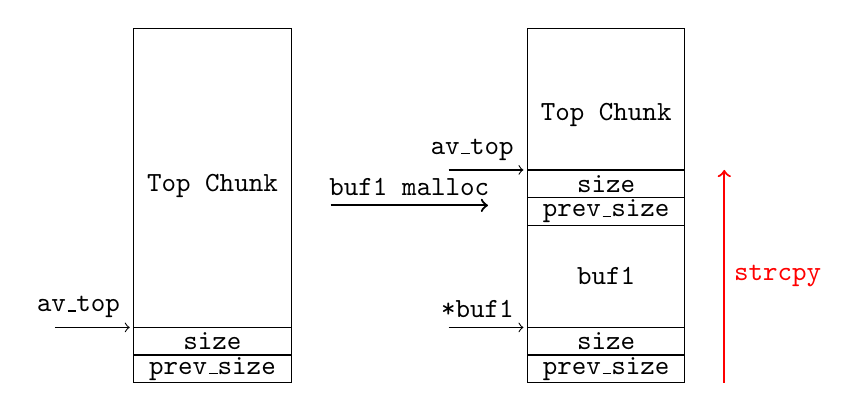
\begin{tikzpicture}[scale=0.5]
		% Draw the main rectangle
		\draw (0,0) rectangle (4,9);
		
		% Draw the divisions
		\draw (0,0.7) -- (4,0.7); % Bottom small section
		\draw (0,1.4) -- (4,1.4); % Middle small section
		
		% Labels
		\node at (2,5) {\texttt{Top Chunk}}; % Large section label
		\node at (2,1.05) {\texttt{size}}; % Middle small section label
		\node at (2,0.35) {\texttt{prev\_size}}; % Bottom small section label
		
		\draw[->] (-2,1.4) -- (-0.1,1.4);
		\node[above left] at (-0.1,1.4) {\texttt{av\_top}};
		
		\draw[thick, ->] (5,4.5) -- (9,4.5);
		\node[above] at (7,4.5) {\texttt{buf1 malloc}};
		
		% Draw the main rectangle
		\draw (10,0) rectangle (14,9);
		
		% Draw the divisions
		\draw (10,0.7) -- (14,0.7); % Bottom small section
		\draw (10,1.4) -- (14,1.4); % Middle small section
		
		\draw (10,4) -- (14,4); 
		\node at (12,2.7) {\texttt{buf1}};
		
		\node at (12,1.05) {\texttt{size}}; % Middle small section label
		\node at (12,0.35) {\texttt{prev\_size}}; % Bottom small section label
		
		\draw (10,4.7) -- (14,4.7); % Bottom small section
		\draw (10,5.4) -- (14,5.4); % Middle small section
		
		\node at (12,5.05) {\texttt{size}}; % Middle small section label
		\node at (12,4.35) {\texttt{prev\_size}}; % Bottom small section label
		
		\node at (12,6.8) {\texttt{Top Chunk}};
		
		\draw[->] (8,1.4) -- (9.9,1.4);
		\node[above left] at (9.9,1.4) {\texttt{*buf1}};
		
		\draw[->] (8,5.4) -- (9.9,5.4);
		\node[above left] at (9.9,5.4) {\texttt{av\_top}};
		
		\draw[red, thick, ->] (15,0) -- (15,5.4);
		\node[red, right] at (15,2.7) {\texttt{strcpy}};
	\end{tikzpicture}
\end{center}

Quindi possiamo arrivare a sovrascrivere la \texttt{size} del top chunk, permettendo di dire al programma quanto spazio libero rimane all'interno. Questa è il primo problema: metadato size del top chunk modificabile dall'attaccante. A questo punto posso "incrementare" la memoria dell'heap (dimensione di \texttt{size}) fino a \textbf{tutta la memoria del processo indirizzabile}, la \texttt{size} è determinata unicamente in modo software. Posso andare ad indirizzare nell'intera memoria del processo.\\

Una volta "allargato tutto", l'attaccante può andare in un punto arbitrario della memoria da sovrascrivere. L'heap adesso include stack, .text ed in generale tutta la memoria. Posso sovrascrivere una zona di memoria arbitraria con un qualsiasi valore. Ad esempio, sovrascrivendo un \texttt{return address} sullo stack.\\

Abbiamo ingannato l'allocatore per \textbf{includere lo stack nello spazio indirizzabile dall'heap}, permettendoci di sovrascrivere una zona di memoria arbitraria.\\

La seconda \texttt{malloc} ha un'ampiezza comandata dall'attaccante, il che ci permette di \textbf{raggiungere la base dello stack}, dove c'è il \texttt{return address} che si vuole sovrascrivere (questa è una dimensione variabile, $\Delta$ tra posizione \texttt{dell'av\_top} e posizione del \texttt{return address}, da calcolare).\\

\newpage

Dopo una \texttt{malloc} di dimensione $\Delta$, l'\texttt{av\_top} sarà nello stack, la terza allocazione di dimensione $n$ (fissa), partirà dall'\texttt{av\_top} (in questo momento stiamo presupponendo non ci siano liste libere, altrimenti bisogna stare un po' più attenti) e quando comincio a scrivere in quest'ultimo buffer (ultima \texttt{strcpy}, comandata dall'attaccante) starò sovrascrivendo il \texttt{return address}, magari con un indirizzo di una zona di memoria il cui contenuto è controllato dall'attaccante (anche nell'heap, generalmente la zona dati non è eseguibile, ma ci sono dei casi in cui potrebbe esserlo).\\

\vfill 

\paragraph{TL;DR:} Inganniamo l'allocatore nel pensare che il top chunk sia più grande di quanto non sia realmente, tramite overflow, per poi andare a sovrascrivere una zona di memoria arbitraria in una scrittura successiva.\\

%Esempi e utilizzo sul link